\chapter{Keko}

Keko on tietorakenne, joka pitää yllä alkioiden kokoelmaa
ja tarjoaa seuraavat operaatiot:

\begin{itemize}
\item lisää alkio kokoelmaan
\item etsi kokoelman pienin/suurin alkio
\item poista kokoelman pienin/suurin alkio
\end{itemize}

Keon operaatioiden toiminta riippuu siitä,
onko keko \emph{minimikeko} vai \emph{maksimikeko}.
Minimikeossa voimme etsiä ja poistaa pienimmän alkion,
kun taas maksimikeossa voimme etsiä ja poistaa suurimman alkion.
Meidän täytyy päättää keon luontivaiheessa,
onko keko minimikeko vai maksimikeko.

Tässä luvussa tutustumme binäärikeko-rakenteeseen,
jossa lisäykset ja poistot vievät aikaa $O(\log n)$
ja haku vie aikaa $O(1)$.
Binäärikeko toteutetaan binääripuun avulla,
ja se on tavallisimmin käytetty kekorakenne.
Javan standardikirjaston tietorakenne prioriteettijono
perustuu binäärikekoon.

\section{Binäärikeko}

Binäärikeko on binääripuu, jonka jokaisessa solmussa on
yksi keossa oleva alkio.
Puu on rakennettu niin, että sen kaikki tasot alinta
tasoa lukuun ottamatta ovat täynnä solmuja,
eli kaikilla solmuilla on vasen ja oikea lapsi.
Alin taso on puolestaan täytetty niin,
että solmut on sijoitettu mahdollisimman vasemmalle
ylempien solmujen lapsiksi.

Keon toiminta perustuu siihen,
että jokainen keon solmu täyttää \emph{kekoehdon}.
Minimikeossa kekoehto vaatii, että jokaisen
solmun arvo on suurempi tai yhtä suuri kuin solmun vanhemman arvo.
Maksimikeossa puolestaan jokaisen solmun arvon tulee olla
pienempi tai yhtä suuri kuin solmun vanhemman arvon.
Kekoehdon ansiosta minimikeon juuressa on keon
pienin alkio ja maksimikeon juuressa on keon suurin alkio.

\begin{figure}
\center
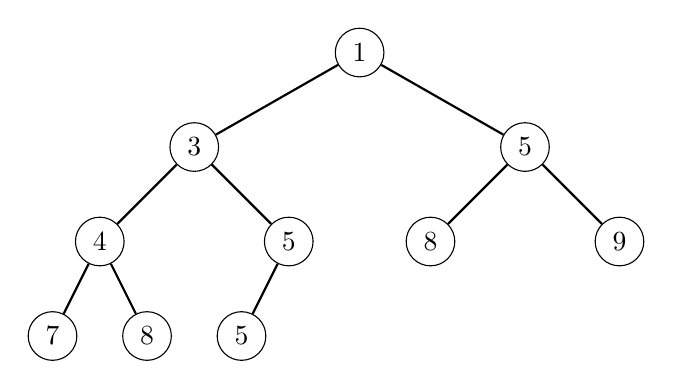
\begin{tikzpicture}[scale=0.6]
\node[draw, circle] (1) at (0,0) {$1$};
\node[draw, circle] (2) at (-3.5,-2) {$3$};
\node[draw, circle] (3) at (3.5,-2) {$5$};
\node[draw, circle] (4) at (-5.5,-4) {$4$};
\node[draw, circle] (5) at (-1.5,-4) {$5$};
\node[draw, circle] (6) at (1.5,-4) {$8$};
\node[draw, circle] (7) at (5.5,-4) {$9$};
\node[draw, circle] (8) at (-6.5,-6) {$7$};
\node[draw, circle] (9) at (-4.5,-6) {$8$};
\node[draw, circle] (10) at (-2.5,-6) {$5$};
\path[draw,thick,-] (1) -- (2);
\path[draw,thick,-] (1) -- (3);
\path[draw,thick,-] (2) -- (4);
\path[draw,thick,-] (2) -- (5);
\path[draw,thick,-] (3) -- (6);
\path[draw,thick,-] (3) -- (7);
\path[draw,thick,-] (4) -- (8);
\path[draw,thick,-] (4) -- (9);
\path[draw,thick,-] (5) -- (10);
\end{tikzpicture}
\caption{Minimikeko, joka sisältää alkiot $[1,3,4,5,5,5,7,8,8,9]$.}
\label{fig:minkek}
\end{figure}


Kuvassa \ref{fig:minkek} on minimikeko,
johon on tallennettu kymmenen alkiota.
Keon kolme ensimmäistä tasoa ovat täynnä
ja neljännellä tasolla kolme ensimmäistä kohtaa on käytetty.
Keon juurena on kokoelman pienin alkio $1$,
ja kaikki solmut täyttävät kekoehdon.
Huomaa, että sama alkio voi esiintyä keossa useasti,
kuten tässä keossa alkiot $5$ ja $8$.

\subsection{Keon tallentaminen}

Tallennamme binäärikeon \emph{taulukkona},
joka sisältää keon solmujen arvot jär\-jestyksessä
ylhäältä alaspäin ja vasemmalta oikealle.
Tämä tehokas tallennustapa on mahdollinen,
koska keon kaikki tasot ovat täynnä solmuja.
Tallennamme keon taulukkoon kohdasta $1$ alkaen,
koska tämä helpottaa keon operaatioiden toteuttamista.

Esimerkiksi tallennamme kuvan \ref{fig:minkek}
keon taulukkona seuraavasti:

\begin{code}
keko = [0,1,3,5,4,5,8,9,7,8,5]
\end{code}

Huomaa, että taulukon ensimmäinen alkio on $0$,
koska emme käytä kohtaa $0$ keon tallentamiseen.

Taulukkototeutuksen etuna on, että voimme laskea
helposti, missä kohdissa keon alkiot ovat taulukossa.
Ensinnäkin keon juuri eli pienin tai suurin alkio
on aina kohdassa $1$.
Lisäksi jos tiedämme, että tietty solmu on kohdassa $k$,
niin solmun vasen lapsi on kohdassa $2k$,
solmun oikea lapsi on kohdassa $2k+1$ ja
solmun vanhempi on kohdassa $\lfloor k/2 \rfloor$.
Esimerkissämme solmu 4
on taulukossa kohdassa $4$,
joten sen vasen lapsi on kohdassa $8$,
oikea lapsi on kohdassa $9$ ja
vanhempi on kohdassa $2$.

Käytännössä haluamme yleensä,
että pystymme lisäämään kekoon uusia alkioita,
jolloin saattaa olla tarpeen suurentaa taulukkoa.
Voimme toteuttaa tämän samalla tavalla kuin taulukkolistassa,
jolloin taulukon suurentaminen ei hidasta keon operaatioita.

\subsection{Operaatioiden toteutus}

On helppoa etsiä minimikeon pienin alkio
tai maksimikeon suurin alkio $O(1)$-ajassa,
koska tämä alkio on aina keon juuressa.
Seuraavaksi näemme, kuinka voimme toteuttaa alkion lisäämisen
sekä pienimmän tai suurimman alkion poistamisen $O(\log n)$-ajassa.

\subsubsection{Alkion lisääminen}

Kun lisäämme uuden alkion kekoon, lisäämme sen ensin seuraavaan
vapaana olevaan paikkaan puussa. Jos alimmalla tasolla on tilaa,
lisäämme sen sinne mahdollisimman vasemmalle,
ja muuten aloitamme uuden tason, jossa on toistaiseksi vain lisättävä solmu.
Alkion lisäämisen jälkeen meidän täytyy varmistaa,
että kekoehto säilyy edelleen voimassa.
Tämä tapahtuu siirtämällä alkiota ylöspäin keossa,
kunnes kekoehto tulee voimaan.

\begin{figure}
\center
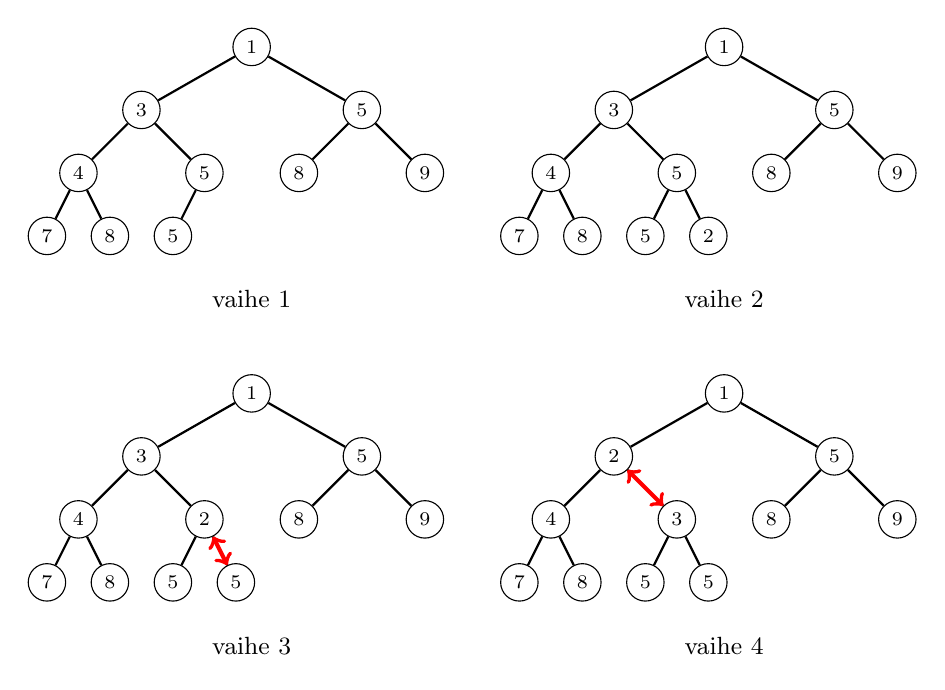
\begin{tikzpicture}[scale=0.4]
\scriptsize
\begin{scope}
\node[draw, circle] (1) at (0,0) {$1$};
\node[draw, circle] (2) at (-3.5,-2) {$3$};
\node[draw, circle] (3) at (3.5,-2) {$5$};
\node[draw, circle] (4) at (-5.5,-4) {$4$};
\node[draw, circle] (5) at (-1.5,-4) {$5$};
\node[draw, circle] (6) at (1.5,-4) {$8$};
\node[draw, circle] (7) at (5.5,-4) {$9$};
\node[draw, circle] (8) at (-6.5,-6) {$7$};
\node[draw, circle] (9) at (-4.5,-6) {$8$};
\node[draw, circle] (10) at (-2.5,-6) {$5$};
\path[draw,thick,-] (1) -- (2);
\path[draw,thick,-] (1) -- (3);
\path[draw,thick,-] (2) -- (4);
\path[draw,thick,-] (2) -- (5);
\path[draw,thick,-] (3) -- (6);
\path[draw,thick,-] (3) -- (7);
\path[draw,thick,-] (4) -- (8);
\path[draw,thick,-] (4) -- (9);
\path[draw,thick,-] (5) -- (10);
\node at (0,-8) {\small vaihe $1$};
\end{scope}
\begin{scope}[xshift=15cm]
\node[draw, circle] (1) at (0,0) {$1$};
\node[draw, circle] (2) at (-3.5,-2) {$3$};
\node[draw, circle] (3) at (3.5,-2) {$5$};
\node[draw, circle] (4) at (-5.5,-4) {$4$};
\node[draw, circle] (5) at (-1.5,-4) {$5$};
\node[draw, circle] (6) at (1.5,-4) {$8$};
\node[draw, circle] (7) at (5.5,-4) {$9$};
\node[draw, circle] (8) at (-6.5,-6) {$7$};
\node[draw, circle] (9) at (-4.5,-6) {$8$};
\node[draw, circle] (10) at (-2.5,-6) {$5$};
\node[draw, circle] (11) at (-0.5,-6) {$2$};
\path[draw,thick,-] (1) -- (2);
\path[draw,thick,-] (1) -- (3);
\path[draw,thick,-] (2) -- (4);
\path[draw,thick,-] (2) -- (5);
\path[draw,thick,-] (3) -- (6);
\path[draw,thick,-] (3) -- (7);
\path[draw,thick,-] (4) -- (8);
\path[draw,thick,-] (4) -- (9);
\path[draw,thick,-] (5) -- (10);
\path[draw,thick,-] (5) -- (11);
\node at (0,-8) {\small vaihe $2$};
\end{scope}
\begin{scope}[yshift=-11cm]
\node[draw, circle] (1) at (0,0) {$1$};
\node[draw, circle] (2) at (-3.5,-2) {$3$};
\node[draw, circle] (3) at (3.5,-2) {$5$};
\node[draw, circle] (4) at (-5.5,-4) {$4$};
\node[draw, circle] (5) at (-1.5,-4) {$2$};
\node[draw, circle] (6) at (1.5,-4) {$8$};
\node[draw, circle] (7) at (5.5,-4) {$9$};
\node[draw, circle] (8) at (-6.5,-6) {$7$};
\node[draw, circle] (9) at (-4.5,-6) {$8$};
\node[draw, circle] (10) at (-2.5,-6) {$5$};
\node[draw, circle] (11) at (-0.5,-6) {$5$};
\path[draw,thick,-] (1) -- (2);
\path[draw,thick,-] (1) -- (3);
\path[draw,thick,-] (2) -- (4);
\path[draw,thick,-] (2) -- (5);
\path[draw,thick,-] (3) -- (6);
\path[draw,thick,-] (3) -- (7);
\path[draw,thick,-] (4) -- (8);
\path[draw,thick,-] (4) -- (9);
\path[draw,thick,-] (5) -- (10);
\path[draw,thick,-] (5) -- (11);
\node at (0,-8) {\small vaihe $3$};
\path[draw,thick,<->,red,line width=1.5pt] (5) -- (11);
\end{scope}
\begin{scope}[yshift=-11cm,xshift=15cm]
\node[draw, circle] (1) at (0,0) {$1$};
\node[draw, circle] (2) at (-3.5,-2) {$2$};
\node[draw, circle] (3) at (3.5,-2) {$5$};
\node[draw, circle] (4) at (-5.5,-4) {$4$};
\node[draw, circle] (5) at (-1.5,-4) {$3$};
\node[draw, circle] (6) at (1.5,-4) {$8$};
\node[draw, circle] (7) at (5.5,-4) {$9$};
\node[draw, circle] (8) at (-6.5,-6) {$7$};
\node[draw, circle] (9) at (-4.5,-6) {$8$};
\node[draw, circle] (10) at (-2.5,-6) {$5$};
\node[draw, circle] (11) at (-0.5,-6) {$5$};
\path[draw,thick,-] (1) -- (2);
\path[draw,thick,-] (1) -- (3);
\path[draw,thick,-] (2) -- (4);
\path[draw,thick,-] (2) -- (5);
\path[draw,thick,-] (3) -- (6);
\path[draw,thick,-] (3) -- (7);
\path[draw,thick,-] (4) -- (8);
\path[draw,thick,-] (4) -- (9);
\path[draw,thick,-] (5) -- (10);
\path[draw,thick,-] (5) -- (11);
\node at (0,-8) {\small vaihe $4$};
\path[draw,thick,<->,red,line width=1.5pt] (2) -- (5);
\end{scope}
\end{tikzpicture}
\caption{Lisäämme alkion 2 kekoon ja nostamme sitä ylöspäin,
kunnes kekoehto tulee jälleen voimaan.}
\label{fig:keklis}
\end{figure}

Kuva \ref{fig:keklis} näyttää, mitä tapahtuu, kun lisäämme
alkion  $2$ esimerkkikekoomme.
Lisäämme alkion ensimmäiseen vapaaseen kohtaan
keon alimmalla tasolla.
Koska alkio 2 on pienempi kuin sen vanhempi 5,
vaihdamme nämä alkiot keskenään.
Tämän jälkeen alkio 2 on pienempi kuin sen vanhempi 3,
joten vaihdamme myös nämä alkiot keskenään.
Nyt kekoehto on voimassa eikä meidän tarvitse enää
tehdä muutoksia kekoon.

Alkion lisääminen kekoon vie aikaa $O(\log n)$,
koska keossa on $O(\log n)$ tasoa ja kuljemme aina
ylöspäin keon pohjalta huippua kohden,
kunnes olemme löytäneet alkiolle sopivan paikan keosta.

\subsubsection{Alkion poistaminen}

Kun haluamme poistaa keon juuressa olevan alkion,
siirrämme ensin keon viimeisen alkion keon juureksi
ja poistamme sille kuuluneen solmun.
Tämän jälkeen lasketamme juureen nostettua alkiota
alaspäin keossa, kunnes kekoehto tulee jälleen voimaan.
Koska solmulla voi olla kaksi lasta,
meillä voi olla kaksi vaihtoehtoa,
kumman lapsista nostamme ylemmäs.
Jos keko on minimikeko, valitsemme lapsen,
jossa on pienempi arvo,
ja jos keko on maksimikeko, valitsemme vastaavasti
lapsen, jossa on suurempi arvo.

\begin{figure}
\center
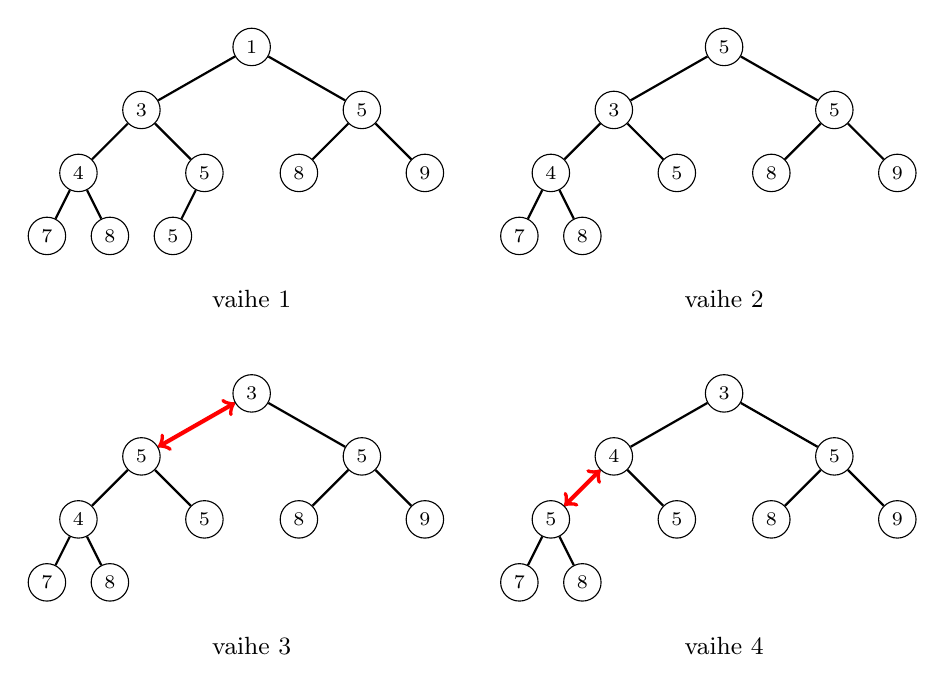
\begin{tikzpicture}[scale=0.4]
\scriptsize
\begin{scope}
\node[draw, circle] (1) at (0,0) {$1$};
\node[draw, circle] (2) at (-3.5,-2) {$3$};
\node[draw, circle] (3) at (3.5,-2) {$5$};
\node[draw, circle] (4) at (-5.5,-4) {$4$};
\node[draw, circle] (5) at (-1.5,-4) {$5$};
\node[draw, circle] (6) at (1.5,-4) {$8$};
\node[draw, circle] (7) at (5.5,-4) {$9$};
\node[draw, circle] (8) at (-6.5,-6) {$7$};
\node[draw, circle] (9) at (-4.5,-6) {$8$};
\node[draw, circle] (10) at (-2.5,-6) {$5$};
\path[draw,thick,-] (1) -- (2);
\path[draw,thick,-] (1) -- (3);
\path[draw,thick,-] (2) -- (4);
\path[draw,thick,-] (2) -- (5);
\path[draw,thick,-] (3) -- (6);
\path[draw,thick,-] (3) -- (7);
\path[draw,thick,-] (4) -- (8);
\path[draw,thick,-] (4) -- (9);
\path[draw,thick,-] (5) -- (10);
\node at (0,-8) {\small vaihe $1$};
\end{scope}
\begin{scope}[xshift=15cm]
\node[draw, circle] (1) at (0,0) {$5$};
\node[draw, circle] (2) at (-3.5,-2) {$3$};
\node[draw, circle] (3) at (3.5,-2) {$5$};
\node[draw, circle] (4) at (-5.5,-4) {$4$};
\node[draw, circle] (5) at (-1.5,-4) {$5$};
\node[draw, circle] (6) at (1.5,-4) {$8$};
\node[draw, circle] (7) at (5.5,-4) {$9$};
\node[draw, circle] (8) at (-6.5,-6) {$7$};
\node[draw, circle] (9) at (-4.5,-6) {$8$};
\path[draw,thick,-] (1) -- (2);
\path[draw,thick,-] (1) -- (3);
\path[draw,thick,-] (2) -- (4);
\path[draw,thick,-] (2) -- (5);
\path[draw,thick,-] (3) -- (6);
\path[draw,thick,-] (3) -- (7);
\path[draw,thick,-] (4) -- (8);
\path[draw,thick,-] (4) -- (9);
\node at (0,-8) {\small vaihe $2$};
\end{scope}
\begin{scope}[yshift=-11cm]
\node[draw, circle] (1) at (0,0) {$3$};
\node[draw, circle] (2) at (-3.5,-2) {$5$};
\node[draw, circle] (3) at (3.5,-2) {$5$};
\node[draw, circle] (4) at (-5.5,-4) {$4$};
\node[draw, circle] (5) at (-1.5,-4) {$5$};
\node[draw, circle] (6) at (1.5,-4) {$8$};
\node[draw, circle] (7) at (5.5,-4) {$9$};
\node[draw, circle] (8) at (-6.5,-6) {$7$};
\node[draw, circle] (9) at (-4.5,-6) {$8$};
\path[draw,thick,-] (1) -- (2);
\path[draw,thick,-] (1) -- (3);
\path[draw,thick,-] (2) -- (4);
\path[draw,thick,-] (2) -- (5);
\path[draw,thick,-] (3) -- (6);
\path[draw,thick,-] (3) -- (7);
\path[draw,thick,-] (4) -- (8);
\path[draw,thick,-] (4) -- (9);
\node at (0,-8) {\small vaihe $3$};
\path[draw,thick,<->,red,line width=1.5pt] (1) -- (2);
\end{scope}
\begin{scope}[yshift=-11cm,xshift=15cm]
\node[draw, circle] (1) at (0,0) {$3$};
\node[draw, circle] (2) at (-3.5,-2) {$4$};
\node[draw, circle] (3) at (3.5,-2) {$5$};
\node[draw, circle] (4) at (-5.5,-4) {$5$};
\node[draw, circle] (5) at (-1.5,-4) {$5$};
\node[draw, circle] (6) at (1.5,-4) {$8$};
\node[draw, circle] (7) at (5.5,-4) {$9$};
\node[draw, circle] (8) at (-6.5,-6) {$7$};
\node[draw, circle] (9) at (-4.5,-6) {$8$};
\path[draw,thick,-] (1) -- (2);
\path[draw,thick,-] (1) -- (3);
\path[draw,thick,-] (2) -- (4);
\path[draw,thick,-] (2) -- (5);
\path[draw,thick,-] (3) -- (6);
\path[draw,thick,-] (3) -- (7);
\path[draw,thick,-] (4) -- (8);
\path[draw,thick,-] (4) -- (9);
\node at (0,-8) {\small vaihe $4$};
\path[draw,thick,<->,red,line width=1.5pt] (2) -- (4);
\end{scope}
\end{tikzpicture}
\caption{Poistamme keon juuressa olevan alkion korvaamalla sen viimeisellä alkiolla
ja laskettamalla sitä alaspäin puussa.}
\label{fig:kekpoi}
\end{figure}

Kuva \ref{fig:kekpoi} näyttää, kuinka poistamme
esimerkkikeostamme pienimmän alkion eli juuressa
olevan alkion 1.
Aluksi korvaamme alkion 1
keon viimeisellä alkiolla 5 ja poistamme keosta
alkiolle 5 kuuluneen solmun.
Tämän jälkeen vaihdamme keskenään alkion 5
ja sen vasemman lapsen alkion 3,
ja sitten vielä alkion 5 ja sen vasemman lapsen alkion 4.
Tämän jälkeen kekoehto on voimassa ja olemme onnistuneet
poistamaan pienimmän alkion keosta.

Alkion poistaminen keosta vie aikaa $O(\log n)$,
koska keossa on $O(\log n)$ tasoa ja kuljemme polkua
alaspäin keon huipulta pohjaa kohden.

\section{Prioriteettijono}

Monissa ohjelmointikielissä kekoa vastaava tietorakenne
tunnetaan nimellä \emph{prioriteettijono}.
Näin on myös Javassa, jonka standardikirjastoon 
kuuluu tietorakenne \texttt{PriorityQueue}.
Se on binäärikekoon perustuva tietorakenne,
joka toteuttaa oletuksena minimikeon.

Seuraava koodi esittelee Javan prioriteettijonon käyttämistä.
Metodi \texttt{add} lisää alkion jonoon,
metodi \texttt{peek} hakee pienimmän alkion
ja metodi \texttt{poll} hakee ja poistaa pienimmän alkion.

\begin{code}
PriorityQueue<Integer> jono = new PriorityQueue<>();
jono.add(5);
jono.add(3);
jono.add(8);
jono.add(7);
System.out.println(jono.peek()); // 3
System.out.println(jono.poll()); // 3
System.out.println(jono.poll()); // 5
\end{code}

Jos haluamme luoda prioriteettijonon, joka onkin
maksimikeko, voimme tehdä sen seuraavaan tapaan:

\begin{code}
PriorityQueue<Integer> jono =
    new PriorityQueue<>(10,Collections.reverseOrder());
\end{code}

Tässä tilanteessa meidän täytyy antaa konstruktorille kaksi tietoa:
keolle alussa muistista varattava tila (tässä 10)
sekä alkioiden järjestämistapa (tässä käänteinen järjestys).
Huomaa, että Java varaa keolle tarvittaessa myöhemmin uuden suuremman muistialueen,
joten tämä määrittely ei tarkoita, että keossa voisi olla enintään 10 alkiota.

Jos haluamme tallentaa \texttt{PriorityQueue}-rakenteeseen omia olioitamme,
meidän tulee toteuttaa luokkaan metodi \texttt{compareTo} ja
merkitä, että luokka toteuttaa rajapinnan \texttt{Comparable}.

\section{Tehokkuusvertailu}

Mitä hyötyä keosta oikeastaan on?
Meillähän on olemassa jo binäärihakupuu,
jonka avulla voimme toteuttaa kaikki keon operaatiot
ja \emph{enemmänkin}.
Keossa voimme hakea ja poistaa vain pienimmän tai suurimman alkion,
mutta binäärihakupuussa voimme käsitellä myös muita alkioita.

Keon etuna on, että siinä on tehokkaan taulukkototeutuksen
ansiosta pienemmät \emph{vakiokertoimet} kuin binäärihakupuussa.
Jos meille riittää, että voimme hakea ja poistaa
vain pienimmän tai suurimman alkion, voi siis olla hyvä
ratkaisu käyttää kekoa binäärihakupuun sijasta.
Mutta kuinka suuria erot ovat käytännössä?

Tämän selvittämiseksi teemme testin,
jossa vertailemme keskenään Javan tietorakenteita
\texttt{PriorityQueue} ja \texttt{TreeSet}.
Testissä meillä on taulukko,
jossa on satunnaisessa järjestyksessä luvut $1,2,\dots,n$.
Lisäämme ensin taulukon $n/2$ ensimmäistä lukua kokoelmaan.
Tämän jälkeen käymme läpi loput $n/2$ lukua,
ja jokaisen luvun kohdalla lisäämme sen kokoelmaan ja
poistamme kokoelman pienimmän luvun.
Laskemme lisäksi samalla summaa poistetuista luvuista.
Käytämme testissä seuraavia koodeja:

\begin{code}
PriorityQueue<Integer> jono = new PriorityQueue<>();
for (int i = 0; i < n/2; i++) {
    jono.add(luvut[i]);
}
long summa = 0;
for (int i = n/2; i < n; i++) {
    jono.add(luvut[i]);
    summa += jono.poll();
}
System.out.println(summa);
\end{code}

\begin{code}
TreeSet<Integer> joukko = new TreeSet<>();
for (int i = 0; i < n/2; i++) {
    joukko.add(luvut[i]);
}
long summa = 0;
for (int i = n/2; i < n; i++) {
    joukko.add(luvut[i]);
    summa += jono.pollFirst();
}
System.out.println(summa);
\end{code}

Taulukko \ref{tab:kekver} näyttää testin tulokset.
Tämän testin perusteella näyttää siltä,
että keon käyttämiseestä on todellista hyötyä,
koska \texttt{PriorityQueue} toimii 2–3
kertaa nopeammin kuin \texttt{TreeSet}.

\begin{table}
\center
\begin{tabular}{rrrr}
taulukon koko $n$ & \texttt{PriorityQueue} & \texttt{TreeSet} \\
\hline
$10^6$ & 0.29 s & 0.78 s \\
$2 \cdot 10^6$ & 0.71 s & 1.50 s \\
$4 \cdot 10^6$ & 1.56 s & 3.72 s \\
$8 \cdot 10^6$ & 3.68 s & 9.43 s \\
\end{tabular}
\caption{Algoritmien suoritusaikojen vertailu.}
\label{tab:kekver}
\end{table}

\section{Lisää keosta}

Käymme seuraavaksi läpi menetelmän, jonka avulla voimme
\emph{muuttaa} taulukon keoksi $O(n)$-ajassa.
Tämän jälkeen luomme katsauksen $O(n \log n)$-aikaiseen
järjestämisalgoritmiin, jonka toiminta perustuu kekoon.

\subsection{Taulukosta keoksi}

Oletetaan, että meillä on $n$ alkiota sisältävä taulukko
ja haluamme muuttaa sen keoksi.
Suoraviivainen tapa on luoda tyhjä keko ja
lisätä jokainen taulukon alkio siihen erikseen $O(\log n)$-ajassa.
Tällä tavalla saamme rakennettua keon $O(n \log n)$-ajassa.
Osoittautuu kuitenkin, että pystymme myös muuttamaan taulukon
\emph{suoraan} keoksi tehokkaammin ajassa $O(n)$.

Ideana on järjestää alkuperäisen taulukon alkioita uudestaan niin,
että kekoehto tulee voimaan taulukon jokaiseen kohtaan --
jolloin taulukko on muuttunut keoksi.
Käymme läpi taulukon alkiot lopusta alkuun ja varmistamme
jokaisessa kohdassa, että kekoehto on voimassa kyseisestä
kohdasta alkavassa alipuussa.
Jos kekoehto ei ole voimassa, korjaamme sen laskettamalla
kyseisen kohdan alkiota alaspäin keossa.
Kun lopulta pääsemme taulukon alkuun, kekoehto on voimassa
koko taulukossa.

\begin{figure}
\center
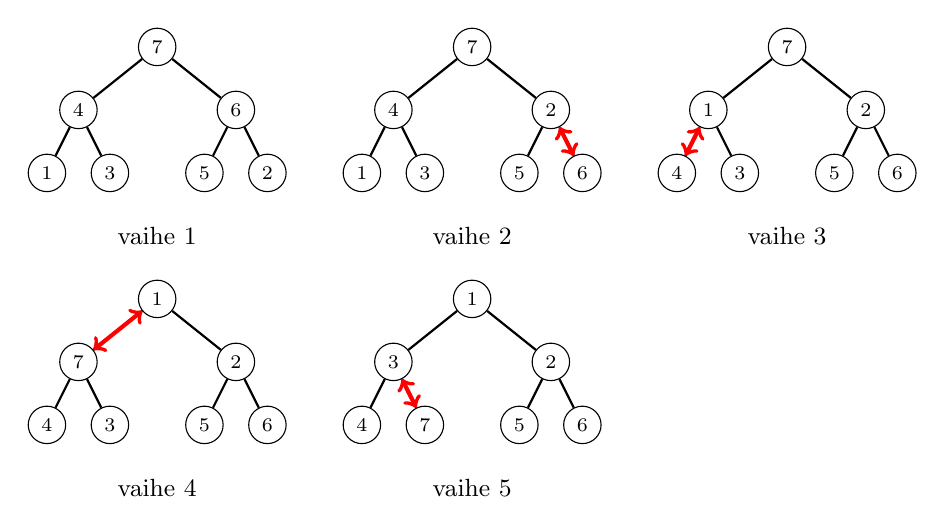
\begin{tikzpicture}[scale=0.4]
\scriptsize
\begin{scope}
\node[draw, circle] (1) at (0,0) {$7$};
\node[draw, circle] (2) at (-2.5,-2) {$4$};
\node[draw, circle] (3) at (2.5,-2) {$6$};
\node[draw, circle] (4) at (-3.5,-4) {$1$};
\node[draw, circle] (5) at (-1.5,-4) {$3$};
\node[draw, circle] (6) at (1.5,-4) {$5$};
\node[draw, circle] (7) at (3.5,-4) {$2$};
\path[draw,thick,-] (1) -- (2);
\path[draw,thick,-] (1) -- (3);
\path[draw,thick,-] (2) -- (4);
\path[draw,thick,-] (2) -- (5);
\path[draw,thick,-] (3) -- (6);
\path[draw,thick,-] (3) -- (7);
\node at (0,-6) {\small vaihe $1$};
\end{scope}
\begin{scope}[xshift=10cm]
\node[draw, circle] (1) at (0,0) {$7$};
\node[draw, circle] (2) at (-2.5,-2) {$4$};
\node[draw, circle] (3) at (2.5,-2) {$2$};
\node[draw, circle] (4) at (-3.5,-4) {$1$};
\node[draw, circle] (5) at (-1.5,-4) {$3$};
\node[draw, circle] (6) at (1.5,-4) {$5$};
\node[draw, circle] (7) at (3.5,-4) {$6$};
\path[draw,thick,-] (1) -- (2);
\path[draw,thick,-] (1) -- (3);
\path[draw,thick,-] (2) -- (4);
\path[draw,thick,-] (2) -- (5);
\path[draw,thick,-] (3) -- (6);
\path[draw,thick,-] (3) -- (7);
\node at (0,-6) {\small vaihe $2$};
\path[draw,thick,<->,red,line width=1.5pt] (3) -- (7);
\end{scope}
\begin{scope}[xshift=20cm]
\node[draw, circle] (1) at (0,0) {$7$};
\node[draw, circle] (2) at (-2.5,-2) {$1$};
\node[draw, circle] (3) at (2.5,-2) {$2$};
\node[draw, circle] (4) at (-3.5,-4) {$4$};
\node[draw, circle] (5) at (-1.5,-4) {$3$};
\node[draw, circle] (6) at (1.5,-4) {$5$};
\node[draw, circle] (7) at (3.5,-4) {$6$};
\path[draw,thick,-] (1) -- (2);
\path[draw,thick,-] (1) -- (3);
\path[draw,thick,-] (2) -- (4);
\path[draw,thick,-] (2) -- (5);
\path[draw,thick,-] (3) -- (6);
\path[draw,thick,-] (3) -- (7);
\node at (0,-6) {\small vaihe $3$};
\path[draw,thick,<->,red,line width=1.5pt] (2) -- (4);
\end{scope}
\begin{scope}[yshift=-8cm]
\node[draw, circle] (1) at (0,0) {$1$};
\node[draw, circle] (2) at (-2.5,-2) {$7$};
\node[draw, circle] (3) at (2.5,-2) {$2$};
\node[draw, circle] (4) at (-3.5,-4) {$4$};
\node[draw, circle] (5) at (-1.5,-4) {$3$};
\node[draw, circle] (6) at (1.5,-4) {$5$};
\node[draw, circle] (7) at (3.5,-4) {$6$};
\path[draw,thick,-] (1) -- (2);
\path[draw,thick,-] (1) -- (3);
\path[draw,thick,-] (2) -- (4);
\path[draw,thick,-] (2) -- (5);
\path[draw,thick,-] (3) -- (6);
\path[draw,thick,-] (3) -- (7);
\node at (0,-6) {\small vaihe $4$};
\path[draw,thick,<->,red,line width=1.5pt] (1) -- (2);
\end{scope}
\begin{scope}[yshift=-8cm,xshift=10cm]
\node[draw, circle] (1) at (0,0) {$1$};
\node[draw, circle] (2) at (-2.5,-2) {$3$};
\node[draw, circle] (3) at (2.5,-2) {$2$};
\node[draw, circle] (4) at (-3.5,-4) {$4$};
\node[draw, circle] (5) at (-1.5,-4) {$7$};
\node[draw, circle] (6) at (1.5,-4) {$5$};
\node[draw, circle] (7) at (3.5,-4) {$6$};
\path[draw,thick,-] (1) -- (2);
\path[draw,thick,-] (1) -- (3);
\path[draw,thick,-] (2) -- (4);
\path[draw,thick,-] (2) -- (5);
\path[draw,thick,-] (3) -- (6);
\path[draw,thick,-] (3) -- (7);
\node at (0,-6) {\small vaihe $5$};
\path[draw,thick,<->,red,line width=1.5pt] (2) -- (5);
\end{scope}
\end{tikzpicture}
\caption{Muutamme taulukon keoksi korjaamalla kekoehdon alipuissa.}
\label{fig:taukek}
\end{figure}

Kuva \ref{fig:taukek} näyttää esimerkin, jossa muutamme taulukon
$[7,4,6,1,3,5,2]$ minimikeoksi.
Kun tulkitsemme taulukon kekona, kekoehto on aluksi
rikki monessa kohdassa taulukossa.
Ensin korjaamme kekoehdon tason 2 alipuissa vaihtamalla
keskenään alkiot 2 ja 6 ja sitten alkiot 1 ja 4.
Tämän jälkeen korjaamme kekoehdon tason 1 alipuussa
eli koko keossa laskettamalla alkion 7 keon huipulta pohjalle.
Nyt kekoehto on voimassa kaikkialla taulukossa,
joten olemme onnistuneet muuttamaan taulukon keoksi.

Miksi sitten tämä vie aikaa vain $O(n)$?
Oletetaan, että keossa on $h$ tasoa ja kaikki
tasot ovat täynnä solmuja, eli keossa on $n=2^h-1$ solmua.
Laskemme jokaiselle tasolle, montako alkiota laskeutuu
enintään jostakin tämän tason solmusta alaspäin.
Ensinnäkin tasolta 1 tasolle 2 laskeutuu enintään 1 alkio --
juuressa oleva alkio.
Vastaavasti
tasolta 2 tasolle 3 laskeutuu enintään $1+2$ alkiota
ja
tasolta 3 tasolle 4 laskeutuu enintään $1+2+4$ alkiota.
Yleisemmin tasolta $k$ tasolle $k+1$ laskeutuu
enintään $1+2+\dots+2^{k-1} = 2^k-1$ alkiota
Koska tasoja on $h$ ja alimmalta tasolta ei voi laskeutua alaspäin,
kokonaistyömäärä on enintään
\[(2^1-1)+(2^2-1)+\dots+(2^{h-1}-1)=2^h-h \le n,\]
joten aikaa kuluu vain $O(n)$.

\subsection{Kekojärjestäminen}

Kekojärjestäminen on järjestämisalgoritmi,
jonka toiminta perustuu kekoon.
Ideana on muuttaa järjestettävä taulukko ensin keoksi
ja sen jälkeen poistaa alkiot keosta yksi kerrallaan
järjestyksessä.
Kekojärjestäminen vie aikaa $O(n \log n)$,
koska taulukon muuttaminen keoksi vie aikaa $O(n)$
ja $n$ alkion poistaminen keosta vie aikaa $O(n \log n)$.

\begin{figure}
\center
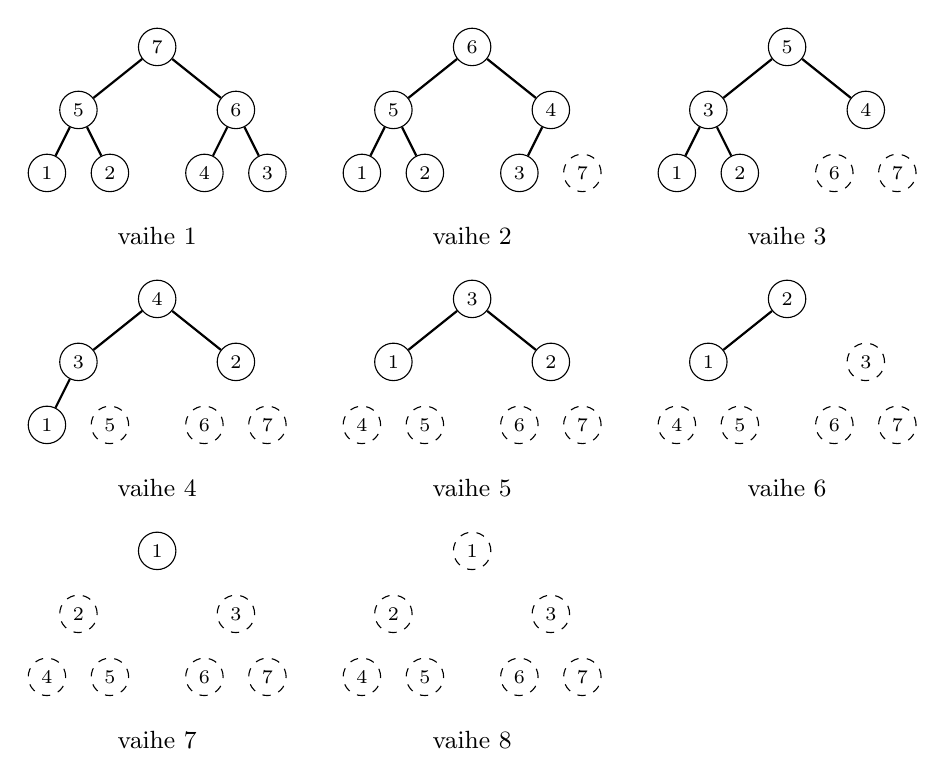
\begin{tikzpicture}[scale=0.4]
\scriptsize
\begin{scope}
\node[draw, circle] (1) at (0,0) {$7$};
\node[draw, circle] (2) at (-2.5,-2) {$5$};
\node[draw, circle] (3) at (2.5,-2) {$6$};
\node[draw, circle] (4) at (-3.5,-4) {$1$};
\node[draw, circle] (5) at (-1.5,-4) {$2$};
\node[draw, circle] (6) at (1.5,-4) {$4$};
\node[draw, circle] (7) at (3.5,-4) {$3$};
\path[draw,thick,-] (1) -- (2);
\path[draw,thick,-] (1) -- (3);
\path[draw,thick,-] (2) -- (4);
\path[draw,thick,-] (2) -- (5);
\path[draw,thick,-] (3) -- (6);
\path[draw,thick,-] (3) -- (7);
\node at (0,-6) {\small vaihe $1$};
\end{scope}
\begin{scope}[xshift=10cm]
\node[draw, circle] (1) at (0,0) {$6$};
\node[draw, circle] (2) at (-2.5,-2) {$5$};
\node[draw, circle] (3) at (2.5,-2) {$4$};
\node[draw, circle] (4) at (-3.5,-4) {$1$};
\node[draw, circle] (5) at (-1.5,-4) {$2$};
\node[draw, circle] (6) at (1.5,-4) {$3$};
\node[draw, circle, dashed] (7) at (3.5,-4) {$7$};
\path[draw,thick,-] (1) -- (2);
\path[draw,thick,-] (1) -- (3);
\path[draw,thick,-] (2) -- (4);
\path[draw,thick,-] (2) -- (5);
\path[draw,thick,-] (3) -- (6);
\node at (0,-6) {\small vaihe $2$};
\end{scope}
\begin{scope}[xshift=20cm]
\node[draw, circle] (1) at (0,0) {$5$};
\node[draw, circle] (2) at (-2.5,-2) {$3$};
\node[draw, circle] (3) at (2.5,-2) {$4$};
\node[draw, circle] (4) at (-3.5,-4) {$1$};
\node[draw, circle] (5) at (-1.5,-4) {$2$};
\node[draw, circle, dashed] (6) at (1.5,-4) {$6$};
\node[draw, circle, dashed] (7) at (3.5,-4) {$7$};
\path[draw,thick,-] (1) -- (2);
\path[draw,thick,-] (1) -- (3);
\path[draw,thick,-] (2) -- (4);
\path[draw,thick,-] (2) -- (5);
\node at (0,-6) {\small vaihe $3$};
\end{scope}
\begin{scope}[xshift=0cm,yshift=-8cm]
\node[draw, circle] (1) at (0,0) {$4$};
\node[draw, circle] (2) at (-2.5,-2) {$3$};
\node[draw, circle] (3) at (2.5,-2) {$2$};
\node[draw, circle] (4) at (-3.5,-4) {$1$};
\node[draw, circle, dashed] (5) at (-1.5,-4) {$5$};
\node[draw, circle, dashed] (6) at (1.5,-4) {$6$};
\node[draw, circle, dashed] (7) at (3.5,-4) {$7$};
\path[draw,thick,-] (1) -- (2);
\path[draw,thick,-] (1) -- (3);
\path[draw,thick,-] (2) -- (4);
\node at (0,-6) {\small vaihe $4$};
\end{scope}
\begin{scope}[xshift=10cm,yshift=-8cm]
\node[draw, circle] (1) at (0,0) {$3$};
\node[draw, circle] (2) at (-2.5,-2) {$1$};
\node[draw, circle] (3) at (2.5,-2) {$2$};
\node[draw, circle, dashed] (4) at (-3.5,-4) {$4$};
\node[draw, circle, dashed] (5) at (-1.5,-4) {$5$};
\node[draw, circle, dashed] (6) at (1.5,-4) {$6$};
\node[draw, circle, dashed] (7) at (3.5,-4) {$7$};
\path[draw,thick,-] (1) -- (2);
\path[draw,thick,-] (1) -- (3);
\node at (0,-6) {\small vaihe $5$};
\end{scope}
\begin{scope}[xshift=20cm,yshift=-8cm]
\node[draw, circle] (1) at (0,0) {$2$};
\node[draw, circle] (2) at (-2.5,-2) {$1$};
\node[draw, circle, dashed] (3) at (2.5,-2) {$3$};
\node[draw, circle, dashed] (4) at (-3.5,-4) {$4$};
\node[draw, circle, dashed] (5) at (-1.5,-4) {$5$};
\node[draw, circle, dashed] (6) at (1.5,-4) {$6$};
\node[draw, circle, dashed] (7) at (3.5,-4) {$7$};
\path[draw,thick,-] (1) -- (2);
\node at (0,-6) {\small vaihe $6$};
\end{scope}
\begin{scope}[xshift=0cm,yshift=-16cm]
\node[draw, circle] (1) at (0,0) {$1$};
\node[draw, circle, dashed] (2) at (-2.5,-2) {$2$};
\node[draw, circle, dashed] (3) at (2.5,-2) {$3$};
\node[draw, circle, dashed] (4) at (-3.5,-4) {$4$};
\node[draw, circle, dashed] (5) at (-1.5,-4) {$5$};
\node[draw, circle, dashed] (6) at (1.5,-4) {$6$};
\node[draw, circle, dashed] (7) at (3.5,-4) {$7$};
\node at (0,-6) {\small vaihe $7$};
\end{scope}
\begin{scope}[xshift=10cm,yshift=-16cm]
\node[draw, circle, dashed] (1) at (0,0) {$1$};
\node[draw, circle, dashed] (2) at (-2.5,-2) {$2$};
\node[draw, circle, dashed] (3) at (2.5,-2) {$3$};
\node[draw, circle, dashed] (4) at (-3.5,-4) {$4$};
\node[draw, circle, dashed] (5) at (-1.5,-4) {$5$};
\node[draw, circle, dashed] (6) at (1.5,-4) {$6$};
\node[draw, circle, dashed] (7) at (3.5,-4) {$7$};
\node at (0,-6) {\small vaihe $8$};
\end{scope}
\end{tikzpicture}
\caption{Esimerkki kekojärjestämisestä.}
\label{fig:kekjar}
\end{figure}

Kuva \ref{fig:kekjar} näyttää esimerkin kekojärjestämisestä,
kun järjestämme taulukon $[5,2,3,1,7,4,6]$
pienimmästä suurimpaan.
Muutamme ensin taulukon maksimikeoksi,
jolloin taulukosta tulee $[7,5,6,1,2,4,3]$.
Tämän jälkeen poistamme yksi kerrallaan
keon juuressa olevan alkion vaihtamalla sen
keon viimeisen alkion kanssa.
Tämän seurauksena keosta poistuneet alkiot
(merkitty katkoviivoilla) muodostavat lopulta järjestetyn taulukon.

Kekojärjestäminen ei ole käytännössä yhtä tehokas algoritmi
kuin lomitusjärjestäminen tai pikajärjestäminen,
minkä vuoksi se ei ole saavuttanut samanlaista asemaa
järjestämisalgoritmien joukossa.
Siinä on kuitenkin yksi kiinnostava ominaisuus:
jos haluamme selvittää vain taulukon $k$ pienintä tai suurinta
alkiota, tämä onnistuu ajassa $O(n+k \log n)$,
koska meidän riittää poistaa keosta $k$ kertaa
pienin tai suurin alkio ajassa $O(\log n)$.